\chapter{\iflanguage{ngerman}{Zukunft}{Future}}
\label{sec:future}
Knowing the current state of miniature robotic systems for medicine, a look into the future is interesting. Many science fiction movies and novels are showing their vision for the medicine of the future. The producers of Star Wars thought of a human like robot equipped with many different miniature tools. The robot is able to replace a hand with a robot hand or removing brain tumors (Fig. \ref{fig:medidroid}). Other novels had the vision of nanobots which are cycling through our bloodstreams. If they find damaged cells or other inner injuries and diseases they would heal or report those (Fig. \ref{fig:nanobot}).
\begin{figure}[H]
    \centering
    \begin{subfigure}[b]{0.2\textwidth}
        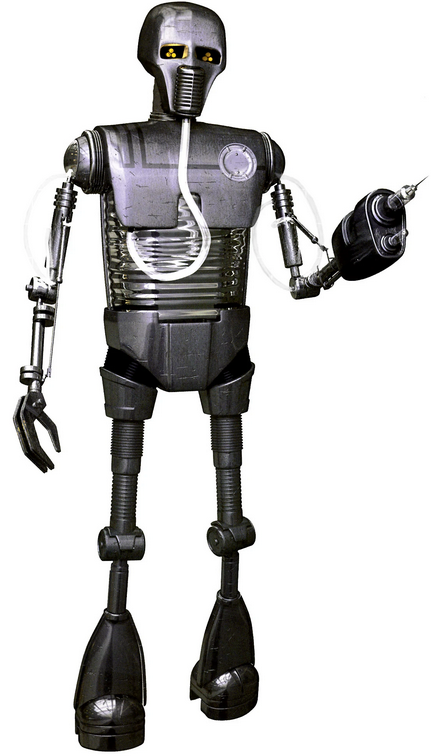
\includegraphics[width=\textwidth]{Figures/starrwars_medidroid.png}
        \caption{Medidroid from Star Wars \cite{medidroid}}
        \label{fig:medidroid}
    \end{subfigure}
    \qquad
    \qquad
    \begin{subfigure}[b]{0.3\textwidth}
        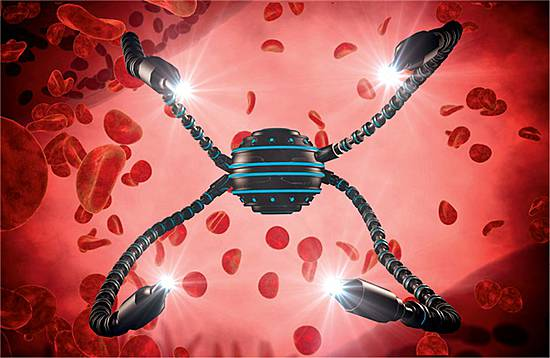
\includegraphics[width=\textwidth]{Figures/nanobot.jpg}
        \caption{Nanobot moving through veins, image from the pharmaceutical press \cite{nanobot}}
        \label{fig:nanobot}
    \end{subfigure}
    \caption{Different kind of science fictional visions of the future of medicine robots}
    \label{fig:visions}
\end{figure}
Fully automated robotic systems are the future due the many advantages against other control systems. Current research are working on automating parts of the robotic system like detection of the tool tip or automated collision avoidance (Sec. \ref{sec:automaticoperation}). When most of the part systems are automated the researches will start to combine the different approaches to build a first fully automated miniature robotic system. A vision like the one of Star Wars is unlikely to come true, because researches are trying to remove restrictions of the human body, like that humans have only 2 hands to use tools. Current robot systems are missing the mobility of the human. That is a part of the Star Wars vision which could become reality. If the robot system would be mobile it could relocate itself to get a better position for reaching a certain area.\\
The earlier a disease is detected the better it can be treated. The best way to detect diseases like a tumor is when the exact corrupted cells are found. For this task a nanobot travelling our blood system like shown in figure \ref{fig:nanobot} is best suited. It would not look like in the picture because the vein system has a diameter of 15\textmu m to 10mm and grippers like in the picture are not possible on this scale. Currently, robot systems are used for automatic colonoscopy. The systems are less painful and also requires less experience from the doctor\cite{automatedColonoscopy}. Additionally, nanobots can be used for delivering drugs into the cells. This is a current research topic \cite{automatedDrugDelivery}. \\ 
The nanobots will not be made of conventional materials but of bio materials. For example it is made of harmless DNA of virus cells. Those nanobots can be used to detect and remove tumor cells \cite{nanobotsOfVirusDNA}. \\